\documentclass[letterpaper]{article}
% The file ijcai13.sty is the style file for IJCAI-13 (same as ijcai07.sty).
\usepackage{ijcai13}
\usepackage{amsmath,amsfonts,amssymb,amsthm}
\usepackage[vlined,algoruled,titlenumbered,noend]{algorithm2e}
\usepackage{array}
\usepackage{epsfig,subfigure}

% Use the postscript times font!
\usepackage{times}

\setlength{\pdfpagewidth}{8.5in}
\setlength{\pdfpageheight}{11in}

\newcommand{\I}{\mathbb{I}}
\newcommand{\casemax}{\mathrm{casemax}}
\newcommand{\casemin}{\mathrm{casemin}}
\newcommand{\UB}{\mathit{UB}}
\newcommand{\LB}{\mathit{LB}}
\newcommand{\Root}{\mathit{Root}}
\newcommand{\Max}{\mathit{Max}}
\def\argmax{\operatornamewithlimits{arg\,max}}
\def\argmin{\operatornamewithlimits{arg\,min}}
\newtheorem*{example*}{Example}

\usepackage{times}
\pdfinfo{ 
/Title (Robust Optimization for Hybrid MDPs with State-dependent Noise) 
/Author (Zahra Zamani, Scott Sanner, Karina Valdivia Delgado, Leliane Nunes de Barros) 
}

% See ../linquad.cameraready/exact_sdp.tex for AAAI-12 Latex source
\title{	Robust Optimization for Hybrid MDPs with State-dependent Noise }

%\author{Anonymous\\
%Paper ID \#1907}%\\

\author{Zahra Zamani\\
ANU \& NICTA\\
Canberra, Australia\\
zahra.zamani@anu.edu.au
\And
Scott Sanner\\
NICTA \& ANU\\
Canberra, Australia\\
ssanner@nicta.com.au
\And
Karina Valdivia Delgado\\
University of Sao Paulo\\
Sao Paulo, Brazil\\
kvd@ime.usp.br
\And
Leliane Nunes de Barros\\
University of Sao Paulo\\
Sao Paulo, Brazil\\
leliane@ime.usp.br}

\begin{document}

\maketitle

\begin{abstract}
Recent advances in solutions to Hybrid MDPs with discrete and
continuous state and action spaces have significantly extended the
class of MDPs for which exact solutions can be derived, albeit at the
expense of a restricted transition noise model.  In this paper, we
work around limitations of previous solutions by adopting a robust
optimization approach in which Nature is allowed to adversarially
determine transition noise within pre-specified confidence
intervals.  This allows one to derive an optimal policy with an
arbitrary (user-specified) level of success probability and
significantly extends the class of transition noise models for which
Hybrid MDPs can be solved.  This work also significantly extends
results for the related ``chance-constrained'' approach in stochastic
hybrid control to accommodate state-dependent noise.  We demonstrate
our approach working on a variety of hybrid MDPs taken from AI
planning, operations research, and control theory, noting that this is
the first time robust solutions with strong guarantees over \emph{all} states
have been automatically derived for such problems.
%%%%%%%%%%%%%%%%%%%%%%%%%%%%%%%%%%%%%%%%%%%%%%%%%%%%%%%%%%%%%%%%%%%%%%
%Continuous spaces with stochastic dynamics can represent a rich class
%of real world problems. While decision theoretic planning provides
%optimal solutions to restricted continuous domains, fully stochastic
%continuous states with continuous action spaces have not been solved
%without approximating techniques. Here we propose a symbolic dynamic
%programming (SDP) approach to provide an optimal closed-form solution
%for Stochastic Discrete and Continuous MDPs with piecewise linear
%dynamics. We show how noisy states are symbolically modelled and
%intuitively minimized in the value iteration algorithm with unknown
%%state parameters. The proposed algorithm uses the extended algebraic
%decision diagrams (XADDs) as an efficient data structure for SDPs to
%demonstrate empirical results on problems such as the Inventory
%Control. The results show the existence of the first fully automated
%exact solution to the stochastic noisy continuous problem definitions.
%%%%%%%%%%%%%%%%%%%%%%%%%%%%%%%%%%%%%%%%%%%%%%%%%%%%%%%%%%%%%%%%%%%%%%
\end{abstract}

\section{Introduction}

Many real-world sequential decision-making problems are naturally
modeled with both discrete and continuous (hybrid) state and action
spaces.  When state transitions are stochastic, these problems can be
modeled as Hybrid Markov Decision Processes (HMDPs), which have been
studied extensively in AI
planning~\cite{boyan01,feng04,li05,kveton06,phase07,hao09,sdp_aaai}
as well as control theory~\cite{Henzinger:1997,Hu:2000,DeSHee:2009}
and operations research~\cite{puterman}.  However, all previous
solutions to hybrid MDPs either take an approximation approach or
restrict stochastic noise on continuous transitions to be
state-independent or discretized (i.e., requiring continuous
transitions to be a finite mixture over deterministic transitions).
% Not mentioning initial state dependence of many control solutions,
% will mention these limitations and inability to handle
% controllability in Related Work.

Unfortunately, each of these assumptions can be quite limiting in
practice when strong \emph{a priori} guarantees on performance are
required in the presence of general forms of state-dependent noise.
For example, in a \textsc{UAV Navigation} problem~\cite{Blackmore:2011}, a human
controller must be aware of all positions from which a UAV with a
given amount of fuel reserves can return to its landing strip with
high probability of success given known areas of (state-dependent)
turbulence and weather events.  In a \textsc{Space Telescope Control}
problem~\cite{DLohr:2012}, one must carefully manage inertial moments and
rotational velocities as the telescope maneuvers between different
angular orientations and zoom positions, where noise margins increase
when the telescope is in unstable positions (extended zooms).  And
in a \textsc{Reservoir Control} problem, one must manage
reservoir levels to ensure a sufficient water supply for a population
while avoiding overflow conditions subject to uncertainty over daily
rainfall amounts.  In all of these problems, there is no room for
error: a UAV crash, a space telescope spinning uncontrollably, or a
flooded reservoir can all cause substantial physical, monetary, and/or
environmental damage.  What is needed are robust solutions to these
problems that are cost-optimal while guaranteed not to exceed a
prespecified margin of error.

To achieve cost-optimal robust solutions we build on ideas
used in the chance-constrained control
literature~\cite{Schwarm:1999,Li:2002,Ono:2008,Blackmore:2011} that
maintain confidence intervals on (multivariate) noise distributions
and ensure that all reachable states are within these noise margins.
However, previous methods restrict either to linear systems with
Gaussian uncertainty and state-independent noise or resort
to approximation techniques.  Furthermore, as these works are all
inherently focused on control from a given initial state, they are
unable to prove properties such as \emph{robust controllability},
i.e., over all states, which have a policy that can achieve a given cost with
high certainty over some horizon?

In this work, we adopt a robust optimization receding horizon control
approach in which Nature is allowed to adversarially determine
transition noise w.r.t. constrained non-deterministic transitions in HMDPs.
This permits us to find robust solutions for a wide range of
non-deterministic HMDPs and allows us to answer questions of \emph{robust
controllability} in very general state-dependent continuous noise settings.
Altogether, this work significantly extends previous results in both
the HMDP literature in AI and robust hybrid control literature
and permits the solution of a new class of robust HMDP control problems.

% What is currently missing are technical claims of novelty: in fact
% all previous operations existed so it's really just the observation
% that they can be combined and used for robust control

\section{Non-deterministic Hybrid MDPs} 

We first formally introduce the framework of Hybrid (discrete and
continuous) Markov decision processes with non-deterministic
continuous noise (ND-HMDPs) by extending the HMDP framework 
of~\cite{sdp_aaai}. A robust solution for this model is then defined
via robust dynamic programming.

\subsection{Factored Representation}

An HMDP is modelled using state variables $(\vec{b},\vec{x}) = (
b_1,\ldots,b_a,x_{1},\ldots,x_c )$ where each $b_i \in \{ 0,1 \}$
($1 \leq i \leq a$) represents a discrete boolean variable and
each $x_j \in \mathbb{R}$ ($1 \leq j \leq c$) is continuous.  To model
continuous uncertainty in ND-HMDPs we additionally define intermediate
noise variables $\vec{n} = n_1, \ldots , n_e$ where each
$n_l \in \mathbb{R}$ ($1 \leq l \leq e$).  Both discrete and
continuous actions are represented in the set $A
= \{a_1(\vec{y}_1), \ldots, a_p(\vec{y}_p) \}$ where each action
$a(\vec{y}) \in A$ references a (possibly empty) vector of continuous
parameters $\vec{y} \in \mathbb{R}^{|\vec{y}|}$; we say an action is
discrete if it has no continuous parameters ($|\vec{y}| = 0$), otherwise
it is continuous.

Given a current state $(\vec{b},\vec{x})$ and next state
$(\vec{b}',\vec{x}')$ and an executed action $a(\vec{y})$ 
at the current state, a real-valued reward function $R(\vec{b},\vec{x},\vec{b}',\vec{x}',a,\vec{y})$
specifies the immediate reward obtained at the current state. The probability of the
next state $(\vec{b}',\vec{x}')$ is defined by a joint state
transition model
$P(\vec{b}',\vec{x}'| \vec{b},\vec{x},a,\vec{y},\vec{n})$ which
depends on the current state, action and noise.
In a factored setting, we do not typically represent the transition
distribution jointly but rather we factorize it into a
dynamic Bayes net (DBN) as follows: %~\cite{dbn}
{\footnotesize
\begin{align}
P&(\vec{b}',\vec{x}'|\vec{b},\vec{x}, a,\vec{y},\vec{n}) = \nonumber  \\
& \prod_{i=1}^a P(b_i'|\vec{b},\vec{x},\vec{b}',\vec{x}',a,\vec{y},\vec{n}) 
  \prod_{j=1}^c P(x_j'|\vec{b},\vec{x},\vec{b}',\vec{x}',a,\vec{y},\vec{n})
\end{align}
}
\emph{Here we allow synchronic arcs among our conditional probabilities 
under the condition that all conditional probabilities in the above DBN form 
a proper directed acyclic graph (DAG)}.
For binary variables $b_i$ ($1 \leq i \leq a$),
$P(b_i'|\vec{b},\vec{x},\vec{b}',\vec{x}',\vec{x},a,\vec{y},\vec{n})$ are defined as
general conditional probability functions (CPFs), which are not necessarily tabular
since they may condition on inequalities of continuous variables.  For
continuous variables $x_j$ ($1 \leq j \leq c$), the CPFs
$P(x_j'|\vec{b},\vec{x},\vec{b}',\vec{x}',a,\vec{y},\vec{n})$ are represented
with \emph{piecewise linear equations} (PLEs) that may have piecewise 
conditions which are arbitrary logical combinations of
$\vec{b}$, $\vec{b}'$ and linear inequalities over $\vec{x}$, $\vec{x}'$,
and $\vec{n}$.  Examples of PLEs follow shortly.

In general, we assume that for each intermediate continuous noise variable 
$n_l$ ($1 \leq l \leq e$)
a non-deterministic noise interval constraint function $N(n_l| \vec{b},\vec{x},a,\vec{y})$ 
has been defined 
that represents a range covering $\alpha$ of the probability mass for $n_l$ and evaluates to 
$-\infty$ for legal values of $n_l$ and $+\infty$ otherwise.  The reason for
the $\pm \infty$ evaluation is simple: 
in a robust solution to HMDPs with non-deterministic noise constraints, Nature will
attempt to adversarially minimize the reward the agent can achieve and hence we let
$N(n_l| \vec{b},\vec{x},a,\vec{y})$ take the value $+\infty$ for illegal values
of $n_l$ to ensure Nature will never choose illegal assignments of $n_l$ when minimizing.

%for an arbitrary constraint set $C(\vec{b},\vec{x},a,\vec{y})$ 
%and 0-1 indicator function $\I$, 
%this can be defined mathematically as:
%\begin{equation}
%N(n_l| \vec{b},\vec{x},a,\vec{y}) = 
%\begin{cases}
%\max_C \I[C\vec{b},\vec{x},a,\vec{y})] \int_{n_l} P(n_l| \vec{b},\vec{x},a,\vec{y}) dn_l > \alpha: & -\infty \\
%\text{otherwise} : & +\infty 
%\end{cases} \label{eq:noise_derivation}
%\end{equation}
As an intuitive example, if 
$P(n_l| \vec{b},\vec{x},a,\vec{y}) = \mathcal{N}(n_l; \mu; \sigma^2)$
is a simple Normal distribution with mean $\mu$ and variance $\sigma^2$ and we let $\alpha = 0.95$ 
then we know that that the 95\% of the probability mass
lies within $\mu \pm 2\sigma$, hence
\begin{equation*}
N(n_l| \vec{b},\vec{x},a,\vec{y}) = 
\begin{cases}
\mu - 2\sigma \leq n_l \leq \mu + 2 \sigma: & -\infty \text{ (legal)}\\
\text{otherwise} : & +\infty \text{ (illegal)}
\end{cases} \; .
\end{equation*}
Of course, there is no requirement for this interval to be symmetric, so there
are technically many ways one could define $N$ to achieve $\alpha=0.95$.  Thus, the 
method for defining $N$ given an $\alpha$ must be specified by the modeler.

%For more general state dependent distributions, ~\eqref{eq:noise_derivation} should
%be evaluated directly; fortunately when the interval constraints $C$ are linear,
%the linear-constrained integration techniques proposed by~\cite{sanner_aaai12} combined
%with the symbolic maximization approach of~\cite{sdp_aaai} often allow this noise function to be 
%computed analytically in closed-form when the indefinite integral over $n_l$ can
%be computed for $N(n_l| \vec{b},\vec{x},a,\vec{y})$ and gradient optimization
%is applied to the result to maximize constraint parameters.

To make the ND-HMDP framework concrete, we now introduce a running example used
throughout the paper:
%%%%%%%%%%%%%%%%%%%%%%%%% ZAHRA TODO
\begin{example*}[\textsc{Reservoir Control}]
The problem of maintaining maximal reservoir levels subject to
uncertain amounts of rainfall is an important problem in operations
research (OR) literature~\cite{Mahootchi2009,Yeh1985}.  In one
variant of this problem, a reservoir operator must
make a daily decision to \emph{drain} some water from a reservoir 
or not subject to weather forecasts over some time horizon.
Specifically in a seven day period, we assume that the weather forecast calls for a 
substantial amount of rain on the fourth day and chances of less rain on the
others.  The objective of the reservoir operator is to avoid underflow or
overflow conditions while maximizing reservoir capacity.

Formally, we assume a state consisting of continuous reservoir level $l_1 \in \mathbb{R}$
and 3 boolean variables $\vec{b}$ to encode a time period of eight days.  We have
two actions $a \in A = \{ \mathit{drain}, \mathit{no}\text{-}\mathit{drain} \}$.
The reward function $R$ is used to prevent overflow and underflow by assigning
$-\infty$ penalty to water levels outside of lower reserve and upper
capacity limits and a reward for the amount of water stored at the end of
the time step.  For both $a \in A$ this is formally defined as:
\vspace{-0mm} 
{\footnotesize
\begin{align}
R(l_1,l_1',\vec{b},\vec{b}',a) &= 
\begin{cases}
(200 \! \leq \! l_1 \! \leq \! 4500) \wedge (200 \! \leq \! l_1' \! \leq \! 4500) & \!\! : l_1'\\
\text{otherwise} & \!\! : -\infty\\
\end{cases} \label{eq:reward}
\end{align}
} 
For the transition function, we assume that on each time step
$\vec{b}' = \vec{b} + 1$ (not shown) and the reservoir level changes
according to the amount of outflow (2000 units of water on a
$\mathit{drain}$ and 0 units on a $\mathit{no}$-$\mathit{drain}$
action) plus a noisy (uncertain) amount of rain $n$: {\footnotesize
\begin{align}
P(l'_1|l_1,n, a& =\mathit{drain}) = \delta \left( l_1'  - (n + l_1 - 2000) \right) \label{eq:drain_trans} \\
P(l'_1|l_1,n, a&=\mathit{no}\text{-}\mathit{drain}) =\delta \left( l_1'  -  (n + l_1) \right) \label{eq:nodrain_trans}
\end{align}}
The use of the $\delta[\cdot]$ function here ensures that the continuous CPF over $l'$ integrates to 1,
which is crucial for defining a proper probability distribution.  While these PLEs are deterministic
note that all continuous noise in this framework enters via the non-deterministic noise variables
in ND-HMDPs.  The noisy level of rainfall $n$ is state-dependent and legal intervals are defined as follows:
{\footnotesize
\begin{align}
N(n|\vec{b},l_1) = \begin{cases}
\vec{b} = 4 \wedge (1200 \leq n \leq 2000) &: -\infty \\
\vec{b} \neq 4  \wedge (0 \leq n \leq 400)&: -\infty \\
\text{otherwise} &: +\infty
\end{cases} \label{eq:noise}
\end{align}}
In short, on day four ($\vec{b} = 4$) the amount of rain is expected to be between
1200 and 2000 units, whereas on the other days it is expected to be between 0 and 400 units.
%%%%%%%%%%%%%%%%%%%%%%%%%%%%%
\end{example*}

%*****

A policy $\pi(\vec{b},\vec{x})$ specifies the action $a(\vec{y}) =
\pi(\vec{b},\vec{x})$ to take at state $(\vec{b},\vec{x})$.  
In a robust solution to HMDPs with non-deterministic noise constraints, 
a sequence of finite horizon policies $\Pi^* = (\pi^{*,1},\ldots,\pi^{*,H})$ is desired such that given the initial state $(\vec{b}_0,\vec{x}_0)$ at $h=0$ and  a discount factor $\gamma, \; 0 \leq \gamma \leq 1$, the expected sum of discounted rewards over horizon $h \in H$ ($H \geq 0$) is maximized subject to Nature's
adversarial attempt to choose value minimizing assignments of the noise variables.  The
value function $V$ w.r.t. $\Pi^*$ in this case is defined via a recursive expectation
{\footnotesize
\begin{align*} 
& V^{\Pi^{*,H}}(\vec{b},\vec{x}) = \min_{\vec{n}} \, \max\!\Big(N(n_1|\vec{b},\vec{x},\Pi^{*,H}),\ldots,\\
& \max\!\Big(N(n_e|\vec{b},\vec{x},\Pi^{*,H}), E_{\Pi^{*,H}} \Big[ r^h \!\! + \! \gamma V^{\Pi^{*,H-1}} \! \! (\vec{b}',\!\vec{x}') \Big| \vec{b}_0,\!\vec{x}_0\Big] \Big) \!\! \cdots \!\! \Big)
\end{align*}}                   
where $r^h$ is the reward obtained at horizon $h$ following policy $\Pi^*$ and using
Nature's minimizing choice of $\vec{n}$ at each $h$.

The effect of ``max'ing'' in each of the previously defined
$N(n_l| \vec{b},\vec{x},a,\vec{y})$ ($1 \leq l \leq e$) with the value
function is one of the major insights and contributions of this paper.
We noted before that Nature will never choose an illegal value of
$n_l$ where $N(n_l| \vec{b},\vec{x},a,\vec{y}) = +\infty$, instead it
will choose a legal value of $n_l$ for which
$N(n_l| \vec{b},\vec{x},a,\vec{y}) = -\infty$ which when ``max'ed'' in
with the value function effectively vanishes owing to the identity
$\max(v,-\infty) = v$.

% B = 1 - H(1-\alpha)
% B - 1 = - H(1-\alpha)
% (B - 1) / -H = 1-\alpha
% (B - 1) / -H - 1 = -\alpha
% 1 + (B - 1) / H = \alpha
% 1 - (1 - B) / H = \alpha
Finally, by leveraging the simple union bound, we can easily prove that
that a policy will achieve $V^{\Pi^{*,H}}$ with at least $1 - H(1-\alpha)$
probability since the probability of encountering a noise value
outside the confidence interval is only $(1-\alpha)$ at any time step.
Hence for a success probability of at least $\beta$, one should choose
$\alpha = 1 - \frac{1 - \beta}{H}$, e.g., $\beta = 0.95$ success probability
requires an $\alpha = 0.99$ for $H=5$.

 
\subsection{Robust Dynamic Programming}

We extend the value iteration dynamic programming
algorithm~\cite{bellman} and specifically the form used for HMDPs
in~\cite{sdp_aaai} to a robust dynamic programming (RDP) algorithm for
ND-HMDPs that may be considered a continuous action generalization of
zero-sum alternating turn Markov games~\cite{littman94}.  Initializing
$V^0(\vec{b},\vec{x}) = 0$ the algorithm builds the $h$-stage-to-go
value function $V^h(\vec{b},\vec{x})$.

The quality $Q_a^{h}(\vec{b},\vec{x},\vec{y},\vec{n})$ of taking
action $a(\vec{y})$ in state $(\vec{b},\vec{x})$ with noise parameters
$\vec{n}$ and acting so as to obtain $V^{h-1}(\vec{b}',\vec{x}')$ thereafter 
is defined as the following:
%\vspace{-4mm}
{\footnotesize
\begin{align}
Q_a^{h}&(\vec{b},\vec{x},\vec{y},\vec{n}) \! = \!
\max\!\Big(\!\!N(n_1|\vec{b},\vec{x},a,\vec{y}),\!\ldots\!, \max\!\Big(\!\!N(n_e|\vec{b},\vec{x},a,\vec{y}), \nonumber \\
& 
\sum_{\vec{b}'} \int \prod_{i=1}^a P(b_i'|\vec{b},\vec{x},\vec{b}',\vec{x}',a,\vec{y},\vec{n}) \!
\prod_{j=1}^c P(x_j'|\vec{b},\vec{x},\vec{b}',\vec{x}',a,\vec{y},\vec{n}) \! \nonumber \\
& \qquad \qquad \; \Big[ R(\vec{b},\vec{x},\vec{b}',\vec{x}',a,\vec{y}) + \gamma V^{h-1}(\vec{b}',\vec{x}') d\vec{x}' \Big] \Big) \! \cdots \! \Big) \hspace{-2mm} \label{eq:qfun}
\end{align}}
Here the noise constraints $N(n_l|\vec{b},\vec{x},a,\vec{y})$ are ``max'ed''
in with the value function to ensure Nature chooses a legal setting 
of $n_l$, thus reducing each $\max$ to an identity operation.  

Next, given $Q_a^h(\vec{b},\vec{x},\vec{y},\vec{n})$ as above for each
$a \in A$, we can proceed to define the $h$-stage-to-go value function
assuming that the agent attempts to maximize value subject to Nature's
adversarial choice of value-minimizing noise:
\vspace{-2mm}
{\footnotesize
\begin{align}
V^{h}(\vec{b},\vec{x}) & = \max_{a \in A} \max_{\vec{y} \in \mathbb{R}^{|\vec{y}|}} \min_{\vec{n} \in \mathbb{R}^{|\vec{e}|}} \left\{ Q^{h}_a(\vec{b},\vec{x},\vec{y},\vec{n}) \right\} \label{eq:vfun}
\end{align}}
The optimal policy at horizon $h$ can also be determined using the
$Q$-function as below:
{\footnotesize
\begin{align}
\pi^{*,h}(\vec{b},\vec{x}) = \argmax_{a \in A}  \argmax_{\vec{y} \in \mathbb{R}^{|\vec{y}|}}  \min_{\vec{n} \in \mathbb{R}^{|\vec{e}|}}  Q^h_a(\vec{b},\vec{x},\vec{y},\vec{n})
\end{align}}
For finite-horizon HMDPs the optimal value function and policy are
obtained up to horizon H.  For infinite horizons where the optimal policy
has finitely bounded value then value iteration terminates when two
values are equal in subsequent horizons ($V^{h} = V^{h-1}$). In this
case $V^\infty = V^h$ and $\pi^{*,\infty} = \pi^{*,h}$.
 
Up to this point we have only provided the abstract mathematical
framework for ND-HMDPs and RDP.  Fortuitously though, all of the
required RDP operations in~\eqref{eq:qfun} and \eqref{eq:vfun} can be
computed exactly and in closed-form as we discuss next.
%We can leverage
%the continuous $\max$ (and analoguously defined $\min$) operations and
%symbolic DP approach of~\cite{sdp_aaai} in order to compute RDP 
%via~\eqref{eq:qfun} and \eqref{eq:vfun} exactly in closed-form.  We
%discuss this next.

\section{Robust Symbolic Dynamic Programming} 

In order to compute the equations above, we propose a \emph{robust
symbolic dynamic programming} (RSDP) approach building on the work
of~\cite{sdp_aaai,sanner_uai11}.  This requires a value iteration
algorithm described in Algorithm~\ref{alg:vi} (\texttt{VI}) and the
regression subroutine described in Algorithm~\ref{alg:regress}.  All
required operations have been previously defined
in~\cite{sdp_aaai,sanner_uai11}.  In what follows we show how these
operations can be used to compute RSDP from the previous section
exactly and in closed-form.

In general we define \emph{all} symbolic functions to be represented
in \emph{case} form~\cite{fomdp} for which a binary ``cross-sum'' operation
can be defined as follows:
%{\footnotesize 
\begin{center}
\begin{tabular}{r c c c l}
&
\hspace{-6mm} 
  $\begin{cases}
    \phi_1: & f_1 \\ 
    \phi_2: & f_2 \\ 
  \end{cases}$
$\oplus$
&
\hspace{-4mm}
  $\begin{cases}
    \psi_1: & g_1 \\ 
    \psi_2: & g_2 \\ 
  \end{cases}$
&
\hspace{-2mm} 
$ = $
&
\hspace{-2mm}
  $\begin{cases}
  \phi_1 \wedge \psi_1: & f_1 + g_1 \\ 
  \phi_1 \wedge \psi_2: & f_1 + g_2 \\ 
  \phi_2 \wedge \psi_1: & f_2 + g_1 \\ 
  \phi_2 \wedge \psi_2: & f_2 + g_2 \\ 
  \end{cases}$
\end{tabular}
\end{center}
%}
%\normalsize
Here $\phi_i$ and $\psi_j$ are logical formulae defined over the state
$(\vec{b},\vec{x})$ and can include arbitrary logical
($\land,\lor,\neg$) combinations of boolean variables
and \emph{linear} inequalities ($\geq,>,\leq,<$) over continuous
variables -- we call this \emph{linear case form} (LCF).  The $f_i$
and $g_j$ are restricted to be \emph{linear} functions.  Similarly
operations such as $\ominus$ and $\otimes$ may be defined with operations
applied to LCF functions yielded LCF results.

In addition to $\ominus$ and $\otimes$, another key binary operation on case
statements the preserves the LCF property is \emph{symbolic case maximization}:

\vspace{-2mm}
{\small
\begin{center}
\begin{tabular}{r c c c l}
&
\hspace{-7mm} $\casemax \Bigg(
  \begin{cases}
    \phi_1: \hspace{-2mm} & \hspace{-2mm} f_1 \\ 
    \phi_2: \hspace{-2mm} & \hspace{-2mm} f_2 \\ 
  \end{cases}$
$,$
&
\hspace{-4mm}
  $\begin{cases}
    \psi_1: \hspace{-2mm} & \hspace{-2mm} g_1 \\ 
    \psi_2: \hspace{-2mm} & \hspace{-2mm} g_2 \\ 
  \end{cases} \Bigg)$
&
\hspace{-4mm} 
$ = $
&
\hspace{-4mm}
  $\begin{cases}
  \phi_1 \wedge \psi_1 \wedge f_1 > g_1    : & \hspace{-2mm} f_1 \\ 
  \phi_1 \wedge \psi_1 \wedge f_1 \leq g_1 : & \hspace{-2mm} g_1 \\ 
  \phi_1 \wedge \psi_2 \wedge f_1 > g_2    : & \hspace{-2mm}f_1 \\ 
  \phi_1 \wedge \psi_2 \wedge f_1 \leq g_2 : & \hspace{-2mm} g_2 \\ 
 \vdots & \vdots
 %\phi_2 \wedge \psi_1 \wedge f_2 > g_1    : & \hspace{-2mm} f_2 \\ 
% \phi_2 \wedge \psi_1 \wedge f_2 \leq g_1 : & \hspace{-2mm} g_1 \\ 
% \phi_2 \wedge \psi_2 \wedge f_2 > g_2    : & \hspace{-2mm} f_2 \\ 
% \phi_2 \wedge \psi_2 \wedge f_2 \leq g_2 : & \hspace{-2mm} g_2 \\ 
  \end{cases}$
\end{tabular}
\end{center}
}
We refer the reader to~\cite{sdp_aaai,sanner_uai11} for further details
on operations required by RSDP.

%%%%%%%%%%%%%%%%%%%%%%%%%%%%%%%%%%%%%%%%%%%%%%%%%%%%%%%%%%%%%%%%%%%%%%%%
\incmargin{.5em}
\linesnumbered
\begin{algorithm}[t!]
\vspace{-.5mm}
\dontprintsemicolon
\SetKwFunction{regress}{Regress}
\Begin{
   $V^0:=0, h:=0$\;
   \While{$h < H$}{
       $h:=h+1$\;
       \ForEach {$a(\vec{y}) \in A$}{
              $Q_a^{h}(\vec{y},\vec{n})\,:=\,$\regress{$V^{h-1},a,\vec{y}$}\;
				$Q_a^{h}(\vec{y}) := \min_{\vec{n}} \, Q_a^{h}(\vec{y},\vec{n})$ $\,$\emph{// noise $\min$}\;
				$Q_a^{h} := \max_{\vec{y}} \, Q_a^{h}(\vec{y})$ $\,$ \emph{// action $\max$}\;
       }
       $V^{h} := \casemax_a \, Q_a^{h}$ $\,$ \emph{// $\max$ over all $Q_a$}\;
       $\pi^{*,h} := \argmax_{(a,\vec{y})} \, Q_a^{h}(\vec{y})$\;
       \If{$V^h = V^{h-1}$}
           {break $\,$ \emph{// Terminate if early convergence}\;}
   }
     \Return{$(V^h,\pi^{*,h})$} \;
}
\caption{\footnotesize \texttt{VI}(CSA-MDP, $H$) $\longrightarrow$ $(V^h,\pi^{*,h})$ \label{alg:vi}}
\vspace{-1mm}
\end{algorithm}
\decmargin{.5em}
%%%%%%%%%%%%%%%%%%%%%%%%%%%%%%%%%%%%%%%%%%%%%%%%%%%%%%%%%%%%%%%%%

%%%%%%%%%%%%%%%%%%%%%%%%%%%%%%%%%%%%%%%%%%%%%%%%%%%%%%%%%%%%%%%%%
\incmargin{.5em}
\linesnumbered
\begin{algorithm}[t!]
\vspace{-.5mm}
\dontprintsemicolon
\SetKwFunction{remapWithPrimes}{Prime}
%\SetKwFunction{sumout}{sumout}

\Begin{
    $Q=$ \remapWithPrimes{$V$} $\,$ \emph{// All $b_i \to b_i'$ and all $ x_i \to x_i'$} \;
%%%%%%%%%%%%%%%%%%% ZAHRA TODO ( check casemax of noise is correct) 
 	\If {$R$ contains primed variables}
	 {$Q := R(\vec{b},\vec{b}',\vec{x},\vec{x}',a,\vec{y}) \oplus (\gamma \cdot Q)$} \;
    \ForEach { $v'$ in $Q$}  
    {
    	\If {$v'$ is $x'_j$}
    	{
    	\emph{// Continuous marginal integration}\\
         $Q := \int Q \otimes P(x_j'|\vec{b},\vec{b}',\vec{x},\vec{x}',a,\vec{y},\vec{n}) \, d_{x'_j}$\;
    	}
	    \If {$v'$ is $b'_i$}
    	{
    	\emph{// Discrete marginal summation}\\
         $Q := \left[ Q \otimes P(b_i'|\vec{b},\vec{b}',\vec{x},\vec{x}',a,\vec{y},\vec{n}) \right]|_{b_i' = 1}$
         \hspace{0mm} \mbox{$\text{\ }$ $\;\;\;\;\;\;$ $\oplus \left[ Q \otimes P(b_i'|\vec{b},\vec{b},\vec{x},\vec{x}',a,\vec{y},\vec{n}) \right]|_{b_i' = 0}$}\;
    	}
    }
    \If {$R$ does not contain primed variables}
    {$Q := R(\vec{b},\vec{x},a,\vec{y}) \oplus (\gamma \cdot Q)$ }\;
     \ForEach { $n_l$ in $Q$}
     {
		\emph{// Sequence of $\max$-in for noise variables}\\          
         $Q(\vec{y},\vec{n}) := \casemax_{n_l} \, ( Q, N(n_l, \vec{b},\vec{x}))$ $\,$ \;
	}
	%%%%%%%%%%%%%%%%%%%%
    \Return{$Q$} \;
}
\caption{\footnotesize \texttt{Regress}($V,a,\vec{y}$) $\longrightarrow$ $Q$ \label{alg:regress}}
\vspace{-1mm}
\end{algorithm}
\decmargin{.5em}
%%%%%%%%%%%%%%%%%%%%%%%%%%%%%%%%%%%%%%%%%%%%%%%%%%%%%%%%%%%%%%%%%

To demonstrate how \texttt{VI} symbolically implements RSDP, we compute $V^1$ for the \textsc{Reservoir Control} example with no boolean variables (assume $\vec{b}=1$). For both actions, the function $Q^1_a$ is computed in line 6 using Alg~\ref{alg:vi}, e.g., this calls Alg~\ref{alg:regress} to compute the following operations for $Q^1_{\mathit{no}\text{-}\mathit{drain}}$:
\begin{itemize}

\item In line 2 of Algorithm~\ref{alg:regress}, we prime $V$ which
  requires a substitution $Q= V \sigma$ where $\sigma = \lbrace
  d_i/d_i' , l_j/l_j' \rbrace$.  Here, $V=V^0=0$ so $Q=V\sigma=0$.

\item Since the reward function contains the primed variable $l_1'$,
  line 4 is performed (and not line 15).  Hence $Q=R\oplus \gamma\cdot 0 = R$
  where $R$ is as defined in~\eqref{eq:reward} with $\vec{b}=1$.

\item For boolean variables, discrete marginalization is performed on
  line 12 using $f|_{b=v}$ (restriction operator) which assigns the
  value $v \in \{ 0,1 \}$ to any occurrence of $b$ in $f$ --- not
  applicable to the example. For continuous variables, line 9 follows
  the rules of integration w.r.t. a $\delta$
  function~\cite{sanner_uai11} which simply yields a symbolic
  substitution: {\footnotesize
\begin{align}
\int f(x'_j) \otimes \delta[x_j' - h(\vec{z})] dx'_j = f(x'_j) \{ x'_j / h(\vec{z}) \}\nonumber
\end{align}}
In the case of the transition for $\mathit{no}\text{-}\mathit{drain}$
in~\eqref{eq:nodrain_trans}, we observe that on integration of $l_1'$,
the only non-zero probability mass occurs when $l_1' = l_1 + n$, 
hence we substitute $l_1'/(l_1 + n)$ wherever
$l_1'$ occurs in our current $Q$ (from line 4, described above).  
This results in the following $Q$ after the for
loop in line 6 of Algorithm~\ref{alg:regress} has completed:
{\footnotesize
\begin{align*}
%Q =   
\begin{cases}
(200 \leq l_1 \leq 4500) \wedge (200 \leq (l_1 + n) \leq 4500) &: \hspace{-1mm} l_1 + n\\
\text{otherwise} &: -\infty\\
\end{cases}
\end{align*}
}
\item In lines 17--20, we 
maximize Q with each of the noise functions $N$ using a sequence of symbolic maximizations. Each noise variable assigns -$\infty$ for legal values of $n_l$ and $+\infty$ for illegal values of $n_l$ defined by the noise model $N(n_l,\vec{b},\vec{x})$. The $Q$ obtained by max'ing in $N(n|\vec{b}=1,l_1)$ from~\eqref{eq:noise} in our running example is 
{\footnotesize
\begin{align*}
%Q =   
\begin{cases}
l_1 \in \mathit{safe} \land (l_1+n) \in \mathit{safe} \land (n \in \mathit{legal}) &: l_1 + n\\
(l_1  \notin \mathit{safe} \lor  (l_1+n) \notin \mathit{safe}) \land (n \in \mathit{legal}) &:  -\infty\\
n \notin \mathit{legal} &: +\infty\\
\end{cases}
\end{align*}
}
where $\mathit{safe}$ water levels correspond to the range [200,4500] and 
$\mathit{legal}$ noise values corresponds to the range [0,400]. 
%The result assigns the value of $l_1+n$ to both safe water levels and legal noise ranges. Unsafe current or next state water levels (with legal noise) lead to -$\infty$ and illegal noise ranges cause the value to be $+\infty$.

\item Next, the regressed $Q_a^{h}(\vec{y},\vec{n})$ from
  Alg~\ref{alg:regress} is minimized over the noise variables
  $\vec{n}$ in line 7 of Alg~\ref{alg:vi}.  Intuitively, this
  continuous minimization will never choose $+\infty$ as there is
  always some legal noise value that can be chosen leading to
  $Q_a^{h}(\vec{y},\vec{n}) < +\infty$.  We refer to~\cite{sdp_aaai}
  for details of continuous variable maximization (from which
  minimization follows).  Even though the minimizing $n$ will be a
  function of $l_1$, for simplicity, let us assume in the first two
  partitions that $n=0$ is the minimizer.  After this substitution and
  $\casemin$'ing (follows from $\casemax$) the partitions together as
  required in the $\min_n$ operation, we obtain the following result:
\begin{align}
Q^1_{\mathit{no}\text{-}\mathit{drain}} =  
\begin{cases}
l_1 \in \mathit{safe}     &: l_1\\
l_1  \notin \mathit{safe} &: -\infty\\
\end{cases} \label{eq:finalq}
\end{align}
Here, we see Nature would have minimized rainfall to minimize reward
and that no $+\infty$ values remain as the $+\infty$ partition was
dominated by other partitions of lesser value after the minimizing
substitution for $n$ and $\casemin$ of all partitions as done in the
$\min_n$ operation.

\item The resulting Q-value with minimal noise would now be maximized over any continuous action parameters (not available in our example) in line 8.  

\item Now we have $Q^1_{\mathit{no}\text{-}\mathit{drain}}$.  Once we
  have obtained $Q^1_{\mathit{drain}}$ in a similar manner (for simplicity,
  let us assume it is the same as~\eqref{eq:finalq} but with $l_1$
  replaced with $l_1-2000$), we would $\casemax$ these two functions
  together to arrive at our final $V^1$:
\begin{align}
V^1 =  
\begin{cases}
(200 \leq l_1 \leq 4500): & l_1 \;\; \hfill (\mathit{no}\text{-}\mathit{drain}) \\
(4500 \leq l_1 \leq 6500): & l_1-2000 \;\; \hfill (\mathit{drain}) \\
\text{otherwise} : & -\infty \;\; \hfill (\mathit{uncontrollable}) \\ 
\end{cases} \nonumber
\end{align}
While we used approximated $Q$-values for space and readability reasons
by making simplifying assumptions (described above), we can still understand
the meaning of the final form of $V^1$.  If the dam levels are high -- we drain,
if lower -- we do not drain.
We remark that the $-\infty$ that occurs here indicates that these 
values of $l_1$ are \emph{not robustly controllable} over a horizon of 1,
i.e., there exist legal choices of noise that occur with probability
greater than $\alpha$ used to define $N$ preventing the agent from
choosing an action that avoids a state trajectory in the illegal
$-\infty$ region defined by the reward.
\end{itemize}

To implement the case statements efficiently with continuous
variables, extended Algebraic Decision diagrams (XADDs) are used from
~\cite{sanner_uai11} extended from ADDs
~\cite{bahar93add}. 

In summary we remark that all operations including the
continuous max and min operations preserve the LCF property,
hence all operations for Robust SDP (RSDP) can be performed exactly in
closed-form -- a novel result for robust solutions to hybrid MDPs
with state-dependent noise.

\section{Empirical Results}

%%%%%%%%%%%%%%%%%%%%%%%%%%%%%%%%%%%%%%%%%%%%%%%%%%%%%%%%%%%%%%%%%%%%%%%%%%
\begin{figure}[tbp!]
%\vspace{-2mm}
\centering

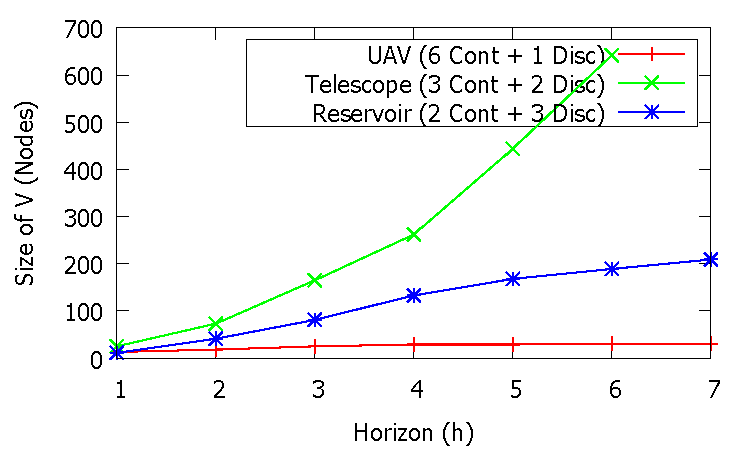
\includegraphics[width=0.42\textwidth]{Figures/Nodes.pdf}\\
\vspace{-3mm}
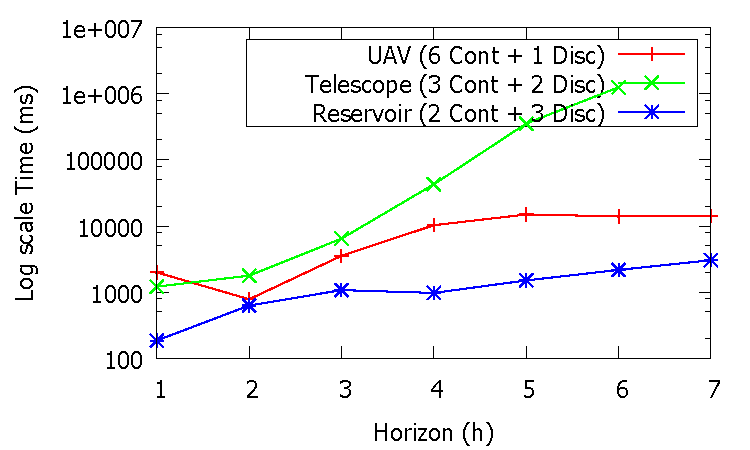
\includegraphics[width=0.42\textwidth]{Figures/Time.pdf}
\vspace{-3mm}
\caption{\footnotesize Space and elapsed time (between current and previous horizon) vs. horizon.
}
\label{fig:SpaceTime}
\vspace{-1mm}
\end{figure}
%%%%%%%%%%%%%%%%%%%%%%%%%%%%%%%%%%%%%%%%%%%%%%%%%%%%%%%%%%%%%%%%%%%%%%%%%%

%%%%%%%%%%%%%%%%%%%%%%%%%%%%%%%%%%%%%%%%%%%%%%%%%%%%%%%%%%%%%%%%%%%%%%%%%%
\begin{figure*}[tbp!]
%\vspace{-2mm}
\centering
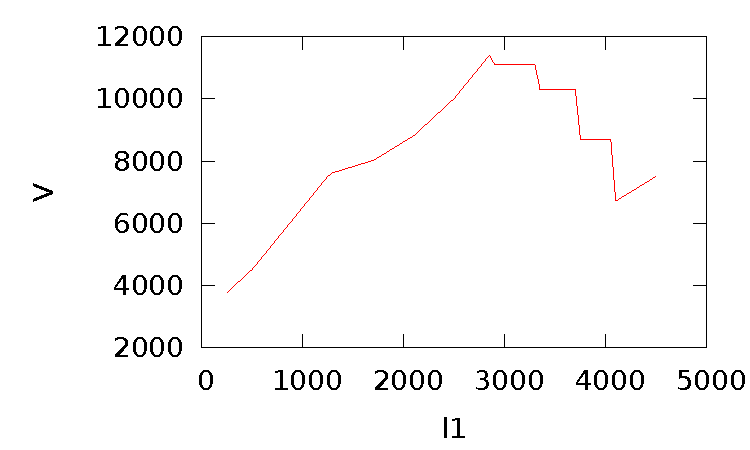
\includegraphics[width=0.33\textwidth]{Figures/reserV7New.pdf}
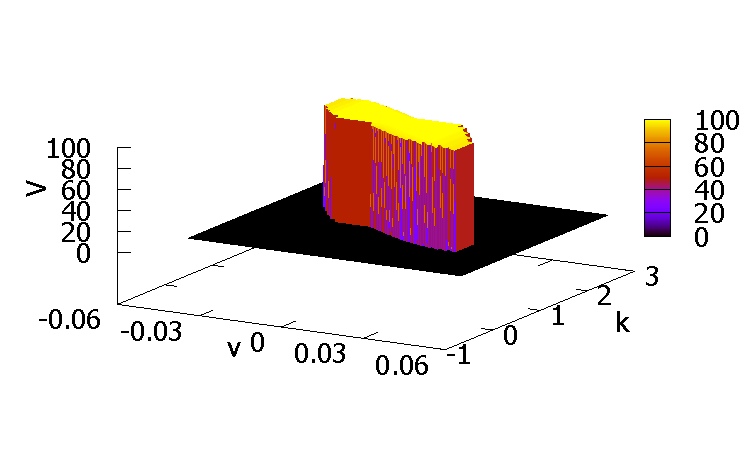
\includegraphics[width=0.33\textwidth]{Figures/telesV4.pdf}
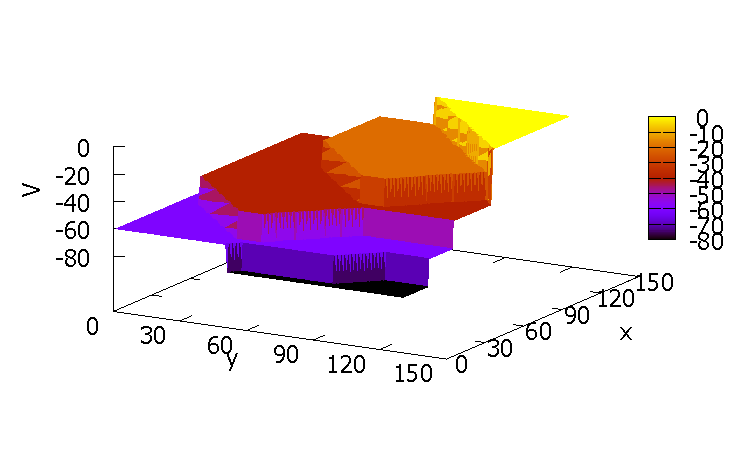
\includegraphics[width=0.33\textwidth]{Figures/uavV4.pdf}
\vspace{-6mm}
\caption{\footnotesize
{\it (left)}  $V^7(l_1,\vec{b}=0)$ \textsc{Reservoir Control} problem;
{\it (middle)} $V^4(k,v,z=true,g=false)$ \textsc{Space Telescope Control} problem; 
{\it (right)}  $V^4(x,y,l=false)$ \textsc{UAV Navigation} problem.
}
\label{fig:Value}
\vspace{-5mm}
\end{figure*}
%%%%%%%%%%%%%%%%%%%%%%%%%%%%%%%%%%%%%%%%%%%%%%%%%%%%%%%%%%%%%%%%%%%%%%%%%%

\label{sec:results}

We evaluated RSDP on the \textsc{Reservoir Control} problem used as a running example,
a \textsc{UAV Navigation} problem  and
a \textsc{Space Telescope Control} problem --- all risk-sensitive
problems as described below.\footnote{All source code and domain definitions
can be found at \texttt{http://code.google.com/p/xadd-inference}.}

Figure \ref{fig:Value} (left) shows the value function for the
\textsc{Reservoir Control} problem in horizon seven. We can observe
that we can gain approximately 11000 units of reward if the reservoir
begins with a water level approximately equal to 3000 at day zero.
Otherwise, a lower initial starting state or the need to drain when
the reservoir is near full lead to lower rewards for all states.
Discontinuities in the value function occur at critical points where
the policy changes over the time horizon.

%{\bf \textsc{Reservoir Control}:} Reservoir management is a well-studied in
%OR~\cite{Mahootchi2009,Yeh1985}.  In this domain we decided between
%\emph{drain} (or \emph{not drain}) each reservoir to maximize
%electricity revenue over the decision-stage horizon while avoiding
%reservoir overflow and underflow.

%We solve a 2-reservoir problem with
%levels $(l_1,l_2)\in [0,\infty]^2$ with reward penalties for
%overflow and underflow and a reward gain of 1, i.e.:


%{\footnotesize
%\begin{align*}
%R & = \begin{cases}
%(l_1 \leq 4500) \wedge (l_2 \leq 4500) \wedge (l_1 \geq 200) \wedge (l_2 \geq 200) &:1\\
%else &: -\infty\\
%\end{cases}
%\end{align*}}


%The electricity is generated in periods when the $\mathit{drain}()$ action
%drains water from $l_2$ to $l_1$, the other action is
%$\mathit{no}$-$\mathit{drain}()$); we assume a daily control,  four days are wet and the next four days are dry (we use three discrete variables to %count the day $d_1$, $d_2$, $d_3$), the rainfall
%replenishment depends on that and is modeled by the noise:
%{\footnotesize
%\begin{align*}
%n & = \begin{cases}
%(d_1) \wedge (n \leq 2000) \wedge (n \geq 1200) &:legal\\
%\neg (d_1) \wedge (n \leq 400) \wedge (n \geq 0) &:legal\\
%else &: illegal\\
%\end{cases}
%\end{align*}}


%The transition function for levels of the $\mathit{drain}$ action are
%{\footnotesize
%\begin{align*}
%l_1' & =(n + l_1 - 2800 + 2000) \\
%l_2'& =(n + l_2 - 2000)
%\end{align*}}
%while for $\mathit{no}$-$\mathit{drain}$ action, the $\mathit{2000}$ term is dropped.

{\bf \textsc{Space Telescope Control}:} We have extended the problem
of slewing a space telescope in order to look a new objective as given
in \cite{DLohr:2012}. This problem has six actions $a_0, \cdots ,a_5$
that change the continuous angle $k$ and angular rate $v$.  The
problem has one boolean state variable $z$ for the telescope zoom
state, one $g$ for reaching the goal state, and one continuous noise
variable.  To model noise in this problem, we have only modified the
transition function for the $a_5$ action in the description
from~\cite{DLohr:2012} (which could not handle noise) to add noise
$n$ when $v < 1$ $\frac{deg}{seg}$ and $z=false$ yielding state
updates for $a_5$ as follows: {\footnotesize
\begin{align*}
k' & =( k + 40.55*v) \\
v'& =(2/3 v + n) \\
z'& =( true ),
\end{align*}}
We model the noise in the transition function of the angular
velocity $v$ for $a_5$ (which changes the zoom of the telescope and for which
the dynamical model is only approximate) as follows:
{\footnotesize
\begin{align*}
n & = \begin{cases}
\neg (z) \wedge (n \leq 0.04*v) \wedge (n \geq -0.04*v) &:-\infty\\
else &: +\infty\\
\end{cases}
\end{align*}}
where we note that noise depends linearly on the angular velocity.

The reward for actions $a_0, \cdots ,a_5$ is given by
{\tiny
\begin{align*}
R & = \begin{cases}
(z) \wedge (v \! \leq \! 0.02) \wedge (k \! \leq \! 1.683) \wedge (v \! \geq \! -0.02) \wedge (k \! \geq \! 1.283) &\!\!:100\\
else &: -\mathit{cost}(a)\\
\end{cases}
\end{align*}}
where the $\mathit{cost}(a)$ of action $a_0$ is 0, $1$ for actions
$a_i$ $i \in \{1,2,3,4\}$ and $10$ for action $a_5$.  
Figure \ref{fig:Value} (middle) shows the value function for the
horizon four. We observe there are states with low angular
rate (approximately $-0.04\leq v \leq 0.04$) that have a policy to
achieve a goal (a reward of 100) with high certainty over this
horizon.

{\bf \textsc{UAV Navigation}:}
In this problem a UAV needs to be able to plan trajectories that take
the aircraft from its current location to a goal given constraints on
time or fuel consumption and known areas of state-dependent turbulence
(e.g., from localized weather events).

The state consists of a UAV´s continuous position $x$ and $y$ and a
boolean variable $l$ indicating whether it has landed.  In a given
time step, the UAV may move a continuous distance $a_x \in [-40,40]$
and $a_y \in [-40,40]$. The turbulence introduces noise $n_x$ and
$n_y$ in the $a_x$ and $a_y$ movements, given by: {\footnotesize
\begin{align*}
n_x & = \begin{cases}
(y \geq 50 + x) \wedge (n_x \leq -20) \wedge (n_x \geq 20) &:-\infty\\
(y < 50 + x) \wedge (n_x \leq -5) \wedge (n_x \geq 5) &:-\infty\\
else &: +\infty\\
\end{cases}\\
n_y & = \begin{cases}
(y \geq 50 + x) \wedge (n_y \leq -20) \wedge (n_y \geq 20) &:-\infty\\
(y < 50 + x) \wedge (n_y \leq -5) \wedge (n_y \geq 5) &:-\infty\\
else &: +\infty\\
\end{cases}
\end{align*}}
The UAV goal is to achieve the region $x+y > 200$. It receives a
reward penalty ($-\infty$) for being in positions from which a UAV
with a given amount of fuel reserves cannot return to its landing
strip with high certainty. 
%added
{\footnotesize
\begin{align*}
R & = \begin{cases}
(l) \wedge (x \leq 130) \wedge (y \leq 130) \wedge (x \geq 0) \wedge (y \geq 0) & \!\! :0\\
(\neg l) \wedge (x \leq 130) \wedge (y \leq 130) \wedge (x \geq 0) \wedge (y \geq 0) & \!\! :-20\\
else &: -\infty\\
\end{cases}
\end{align*}}
If the UAV is not in the goal position ($\neg l$), the action
reward is a cost of -20 fuel units for the given time period.  We note that
with six continuous variables in the regression (2 state, 2 action, 2 noise),
this problem is relatively high-dimensional and could not be easily solved
via discretization methods, which also incur approximation error not encountered
in our exact solution provided here.

Figure \ref{fig:Value} (right) shows the \emph{converged} value
function for a horizon of four time steps showing the 
relative cost of returning to the landing strip from different
positions with lower values near high levels of turbulence.

\textbf{Time and Space:} Figure \ref{fig:SpaceTime} shows the time and
space for each of the solved problems.  The \textsc{UAV Navigation}
problem has more continuous variables, however we can see that it is
easier to solve than the \textsc{Space Telescope Control}, one
possible reason is that the latter has more actions with more
complex forms of linearly state dependent noise.

\section{Related Work}

%%HYBRID SYSTEMS

% We focus on controllability in stochastic systems... few results
% here except in chance-constrained systems where only
% approximate solutions are determined or dynamics
% is restricted to be Gaussian with state-independent noise.
% We argue that finding optimal solutions with exact guarantees
% on controllability in systems with state-dependent noise is
% crucial in settings like autonomous vehicles, satellite manuevers,
% and environmental control systems.

This work extends results in HMDP in AI
~\cite{boyan01,feng04,li05,kveton06,phase07,hao09,sdp_aaai} and hybrid
system control literature~\cite{Henzinger:1997,Hu:2000,DeSHee:2009}
to handled state-dependent noise.

In the hybrid control literature, a challenging topic is to solve the
controllability problem that is NP hard \cite{Blondel:1999}. A hybrid
system is called hybrid controllable if, for any pair of valid states,
there exists at least one permitted control sequence (correct
control-laws) between them \cite{Tittus:1998,Yang:2007}.  Another
challenging topic for stochastic hybrid systems, a class of hybrid
systems that allows uncertainty, is tried to maximize the probability
that the execution will remain in safe states as long as
possible \cite{Hu:2000}.  This work is related with both topics,
however we want to answer a slightly different question, called the
robust controllability problem: what states have a policy to achieve a
goal (that can be modeled as a reward or cost function) with high
certainty over some horizon?  To the authors’ knowledge, in the
control area there are few results to answer a similar question except
in the chance-constrained predictive stochastic sub-area, that finds
the optimal sequence of control inputs subject to the constraint that
the probability of failure must be below a user-specified
threshold \cite{Blackmore:2011}. However all the previous work in this
sub-area is focused on linear systems subject to Gaussian uncertainty
and state-independence
noise \cite{Schwarm:1999,Li:2002,Ono:2008,Blackmore:2011} or resort to
approximation techniques \cite{Blackmore:2010}.  We note that 
our approach is not approximate and can provably provide robust solutions to problems with
state-dependent noise in a receding horizon control framework that
answers the robust controllability question for \emph{all} states.

\section{Concluding Remarks}

% In results, need to point out that for larger problems, reasonable
% discretizations into 100 intervals per variable could lead to
% (10^2)^6 = 10^12 = 1 trillion states that would prohibit the
% application of even one Bellman backup.  This solution is exact to
% arbitrary precision and does not introduce additional errors owing
% to discretization noise.
%
% Should mention somewhere modifications to max operator to handle
% negative values and important order of operations when working
% with infinities (0*anything=0) so cannot terminate early when
% see a 0 on a branch during Apply.
%
% Future work: hierarchy and decompositions with bounds, RTDP, 
%              UCT and sampling, determinization-discretization 
%              guided solutions, reward shaping, upper and lower
%              bounds and refining solutions, nonlinear by adaptive 
%              linearization, bounded approximations, extensions 
%              beyond piecewise linear to bilinear, quadratic, and 
%              beyond, conversion to polygons and GPU computation
%              -- or just keep polytopes -- key is parrallelization,
%              exploit more structure on min/max and integrate --
%              more efficient than for every path?  policy iteration
%              and finite state controllers; policy constraints
%              reduce points for expensive (continuous) maximization.
%              Concurrent multiagent zero-sum conditioned on 
%              continuous state.  Aync. VI by backing up state with
%              largest bound gap, or Bounded Cont. RTDP.
%              Can handle nonlinear with RTDP... instantiate state
%              prior to backup!!!

This work has combined symbolic techniques from
the HMDP literature in AI with techniques from chance-constrained
control theory to find provably robust solutions over \emph{all} states
on problems with piecewise linear transitions and state-dependent noise
for which no general exact closed-form solutions previously existed.
%Using these techniques we were able to find optimal policies and
%answer questions of robust controllability for a variety of highly
%risk-sensitive applications from AI planning, control theory, and
%operations research such as \textsc{UAV Navigation}, \textsc{Space
%  Telescope Control}, and \textsc{Reservoir Control}.  
For future work, combining RSDP with
search techniques as in HAO*~\cite{hao09} will preserve 
robust optimality guarantees for a set of initial states while
substantially increasing scalability.  Furthermore,
~\cite{Ono:2008} observe that the probability of failure
(risk) need not be allocated uniformly at each decision stage --- we
can dynamically allocate risk over decisions to achieve
robust controllability for a larger set of states.

{\footnotesize
\section*{Acknowledgements}

NICTA is funded by the Australian Government as represented by
the Department of Broadband, Communications and the Digital
Economy and the Australian Research Council through the ICT
Centre of Excellence program.
}

%\appendix

%% The file named.bst is a bibliography style file for BibTeX 0.99c
\bibliographystyle{named}
\bibliography{hybnoise}

\end{document}

